\section{Breast cancer}
\label{sec:brca}

Breast cancer remains a major challenge in contemporary healthcare, being the
most frequently diagnosed cancer among women worldwide.
In 2022, approximately 2.3 million new cases were recorded, along with 666,000
deaths, highlighting its impact as a critical public health issue.
That year, breast cancer accounted for 26.2\% of all cancer diagnoses in
women\supercite{bray_global_2024,ferlay_global_2024}.
As shown in \cref{fig:brca_incidence_mortality}, breast cancer is the cancer
type with the highest incidence and the highest mortality rate in women.

Projections indicate that by 2070, the incidence could rise to 4.4 million
cases, placing an increasing strain on healthcare
systems\supercite{lei_global_2021}.

\begin{figure}[ht] \begin{tabular}{cc} \begin{subfigure}{0.5\textwidth}
            \centering

            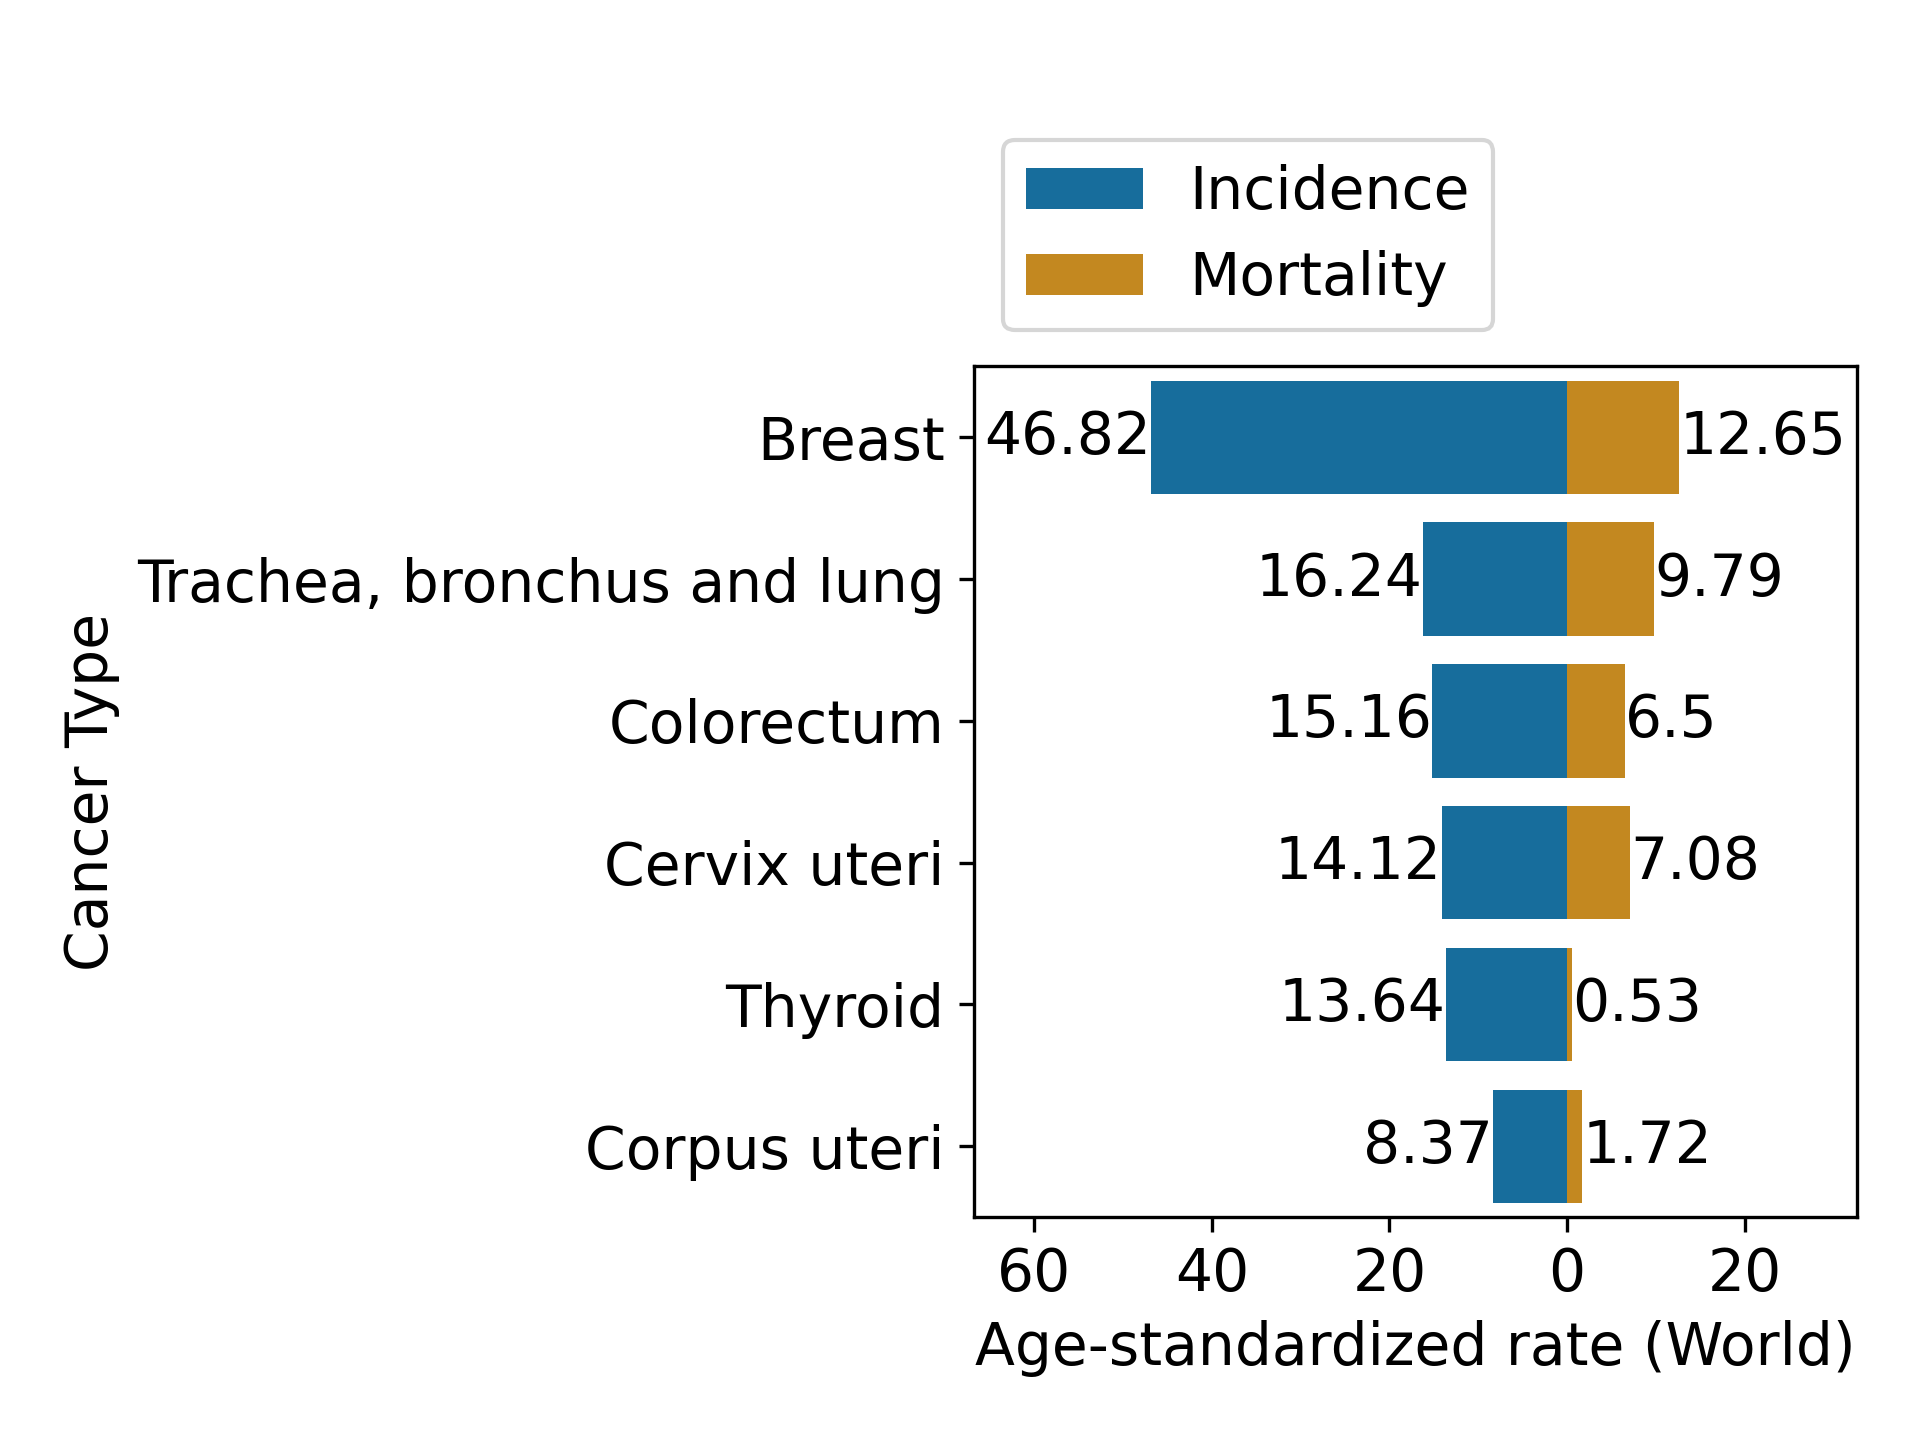
\includegraphics[width=\linewidth]{chapters/2_background/figures/bar.png}
            \caption{Incidence and mortality of cancer types}
            \label{fig:brca_bar}
        \end{subfigure} & \begin{subfigure}{0.5\textwidth} \centering

            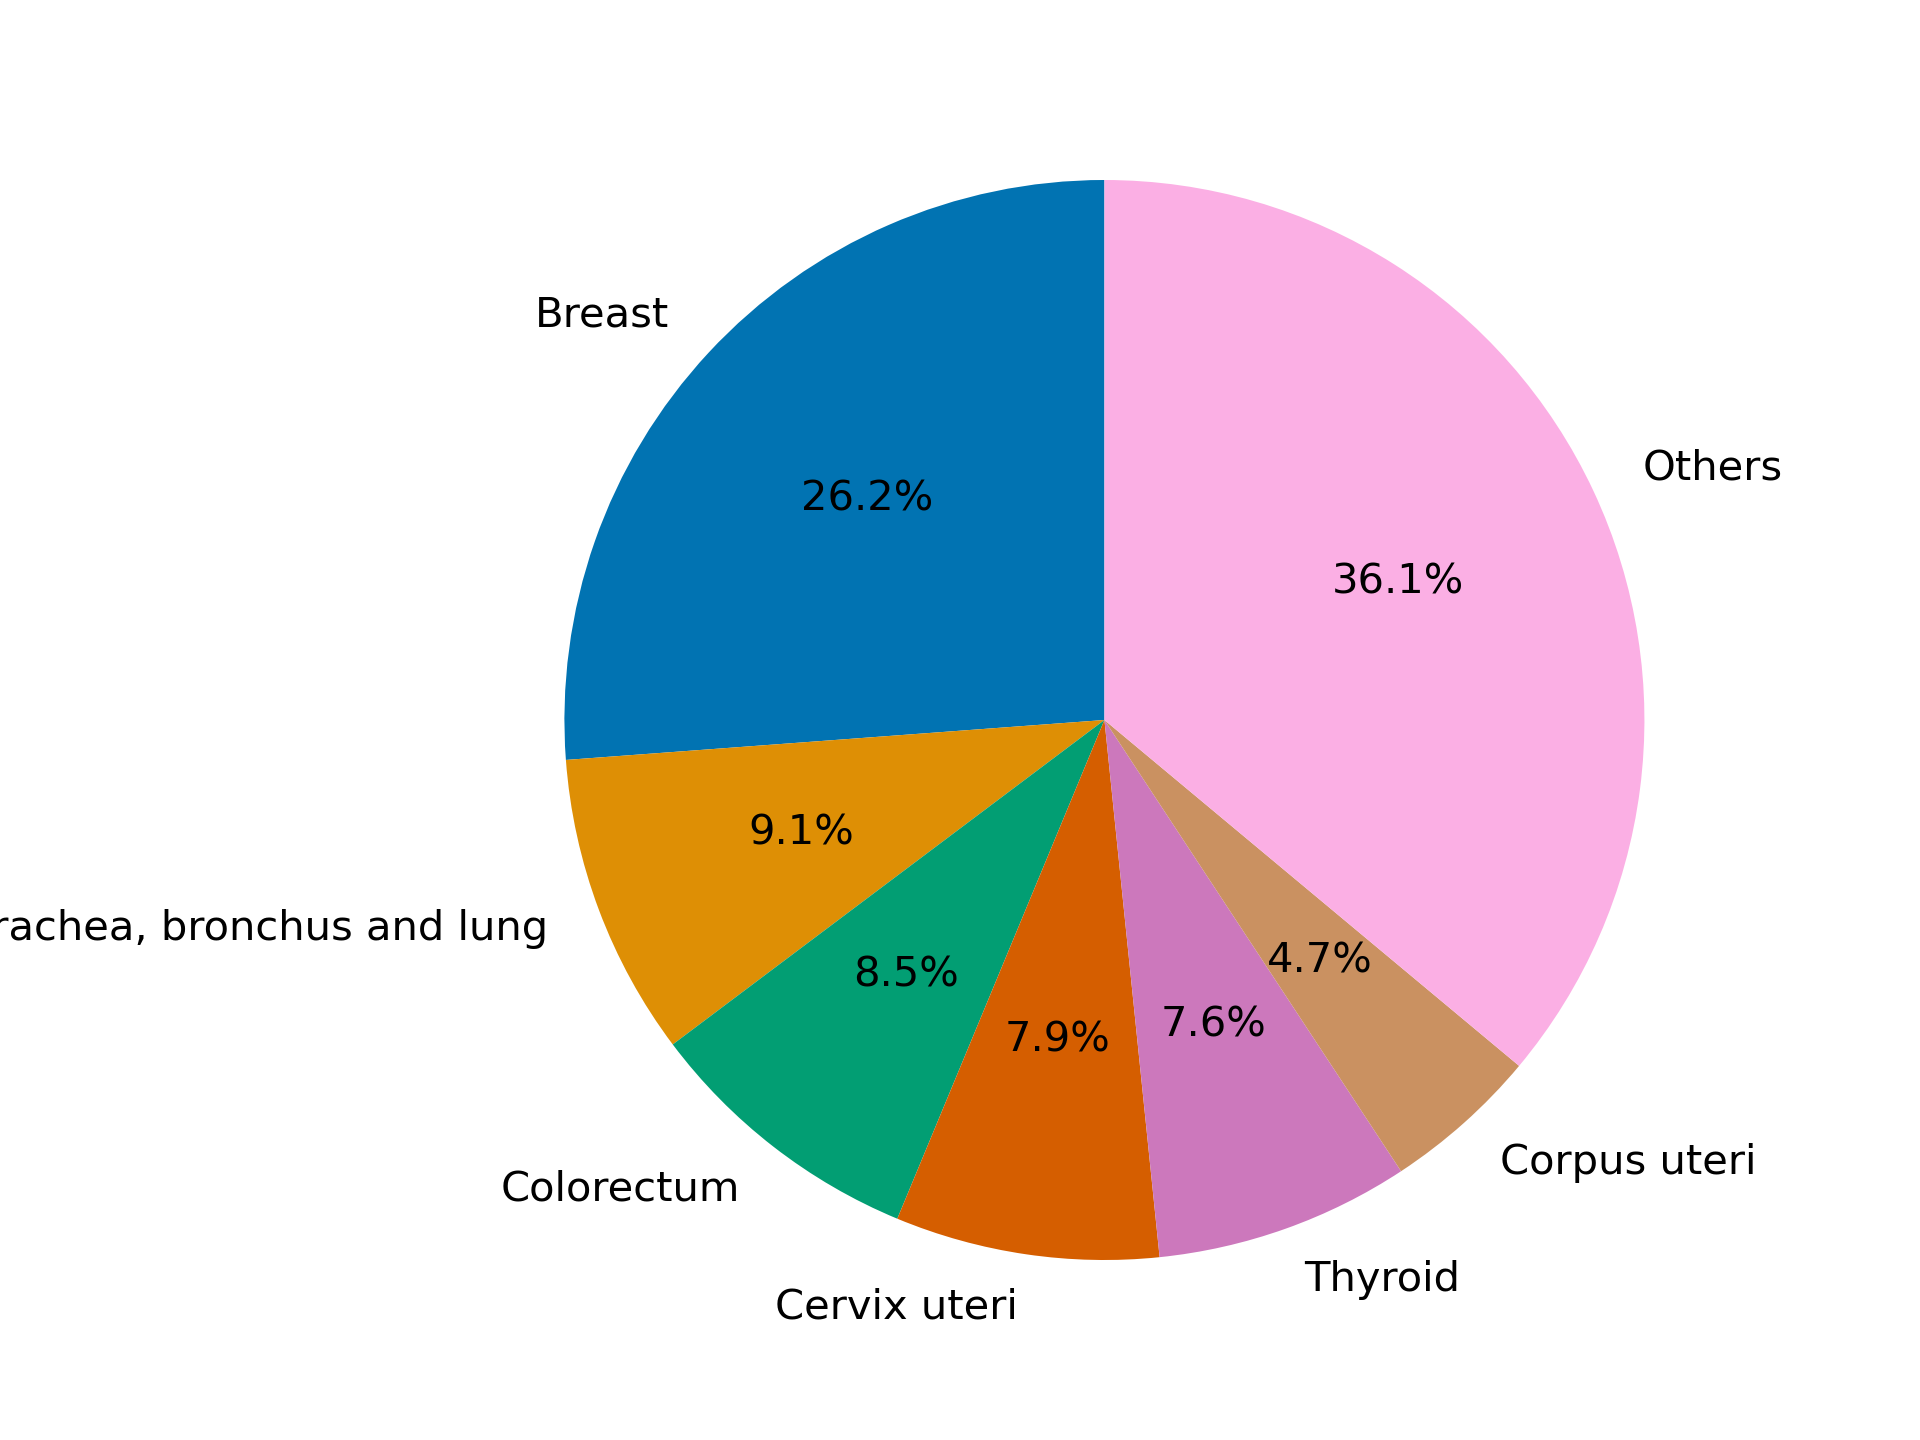
\includegraphics[width=\linewidth]{chapters/2_background/figures/pie.png}
            \caption{Relative incidence of cancer types}
            \label{fig:brca_pie}
        \end{subfigure} \end{tabular} \caption{Overview of the cancer types
        with the highest global incidence in women in 2022.
        Data were obtained from the Global Cancer Observatory
        \supercite{bray_global_2024,ferlay_global_2024}.
        Both subplots show the 6 cancer types with the highest incidence \gls{asr}.
        The numbers represent the \gls{asr} of incidence and mortality per 100,000
        individuals.
        Age standardization is necessary when comparing populations with different age
        structures\supercite{segi_age-adjusted_1960,doll_cancer_1966}.
        \textbf{a}: Absolute incidence and mortality values.
        Breast cancer is the cancer type with the highest incidence and the highest
        mortality rate with an incidence \gls{asr} of 46.82 and a mortality \gls{asr}
        of 12.65.
        \textbf{b}: Relative incidence \gls{asr} values.
        Breast cancer makes up 26.2\% of all newly diagnosed cancer cases.
    }
    \label{fig:brca_incidence_mortality} \end{figure}

Despite advancements in treatment and early detection, disparities in access to
care and late-stage diagnoses remain prevalent, particularly in low-resource
settings\supercite{wilkinson_understanding_2022,ginsburg_breast_2020}.
The mortality \gls{asr} from breast cancer is approximately 12.65 per 100,000
women per year, reflecting the ongoing challenges in managing this complex
disease \supercite{bray_global_2024,ferlay_global_2024}.
Thus, breast cancer continues to pose a formidable challenge, necessitating
concerted efforts in research, awareness, and healthcare delivery to improve
outcomes\supercite{desantis_breast_2019}.

\subsection{Types}
\label{sec:brca_types}

Breast cancer is a heterogeneous disease characterized by various subtypes that
differ in their molecular features, clinical behavior, and response to
treatment\supercite{harbeck_breast_2019}.
The classification of breast cancer is primarily based on the expression of
\glspl{hr}, such as estrogen and progesterone, and the \gls{her2}.
Understanding these subtypes is crucial for determining prognosis and tailoring
treatment strategies.
One of the most common classifications is based on hormone receptor status,
which divides breast cancer into three main categories: \gls{hr+}, \gls{her2+},
and \gls{tnbc}\supercite{clusan_basic_2023}.

\subsubsection{\Glsfmtfull{hr+}}
\gls{hr+} breast cancers express either \glspl{er} or \gls{pr} and
are typically treated with hormone therapies such as \gls{tam} or aromatase
inhibitors such as \gls{let}\supercite{geyer_molecular_2012}.
Within the \gls{hr+} category, there are further distinctions, such as luminal
A and luminal B subtypes.
Luminal A tumors are generally associated with a better prognosis and lower
proliferation rates, while luminal B tumors tend to be more aggressive and may
require chemotherapy in addition to hormone
therapy\supercite{geyer_molecular_2012}.

\subsubsection{\Glsfmtfull{her2+}}
\Gls{her2+} breast cancer is characterized by overexpression of the \gls{her2}
protein, which is associated with aggressive disease and poorer outcomes if
untreated.
However, the advent of targeted therapies, such as trastuzumab, has
significantly improved survival rates for patients with \gls{her2+} breast
cancer\supercite{modi_antitumor_2020}.
Recent studies have also identified a subset of \gls{her2}-low breast cancer,
which may not meet the criteria for \gls{her2} positivity but still expresses
low levels of the \gls{her2} protein.
This subtype has been shown to have distinct clinical outcomes and may benefit
from specific therapeutic
approaches\supercite{won_clinical_2022,mutai_prognostic_2021}.

\subsubsection{\Glsfmtfull{tnbc}}
\Gls{tnbc} is defined by the absence of \gls{er}, \gls{pr},
and \gls{her2} expression.
This subtype is known for its aggressive nature and limited treatment options,
as it does not respond to hormone therapies or \gls{her2}-targeted
therapies\supercite{sizemore_triple_2021}.
\Gls{tnbc} can be further classified into several subtypes based on gene
expression
profiles, including basal-like and claudin-low subtypes, which exhibit
different biological behaviors and responses to
treatment\supercite{lehmann_identification_2011}.
The lack of targeted therapies for \gls{tnbc} has led to ongoing research into
novel treatment strategies, including immunotherapy and combination
therapies\supercite{lehmann_identification_2011}.

\begin{table}[ht]
    \centering
    \begin{tabular}{|l|c|c|c|c|}
        \hline
                                        & \makecell{\gls{hr+}
        \\Luminal A} &
        \makecell{\gls{hr+}                                                  \\
        Luminal B}
                                        &
        \gls{her2+}
                                        & \gls{tnbc}
        \\ \hline
        Proportion of cases             & 60\%                & 10\%
                                        &
        20\%
                                        & 10\%
        \\
        \gls{er}\textalpha{} expression & ++                  & +
                                        & -
                                        & -
        \\
        PR expression                   & ++                  & +
                                        & -
                                        & -
        \\
        \gls{her2} expression           & -                   & +/-
                                        & +
                                        & -
        \\
        Proliferation (Ki67)            & Low                 & High
                                        &
        High
                                        & High
        \\
        Prognosis                       & Good                & Intermediate
                                        &
        Intermediate
                                        & Poor
        \\
        Therapy                         & Endocrine           & Endocrine

                                        &
        Anti-\gls{her2}
                                        & Chemotherapy
        \\ \hline
    \end{tabular}
    \caption{Characteristics of breast cancer
        types\supercite{clusan_basic_2023}.
        \Gls{hr+}, especially the luminal A subtype, is the most
        abundant type of breast cancer.
        \Gls{her2+} and \gls{tnbc} are less common
        but are associated with more aggressive disease and poorer outcomes.
        The table shows the main characteristics of each subtype, including \gls{hr}
        expression, \gls{her2} status, proliferation rates, prognosis, and treatment
        options.
        More information about treatment options can be found in
        \cref{sec:brca_treatment}.
    }
    \label{tab:brca_subtypes}
\end{table}

\subsection{Causes and risk factors}
\label{sec:brca_risk-factors}

Breast cancer is a complex disease, with various causes and risk factors.
Understanding these factors is key to improving prevention, early detection,
and treatment.
These risk factors can generally be grouped into genetic, lifestyle,
environmental, and — most relevant to this thesis — hormonal
influences\supercite{clusan_basic_2023}.

\paragraph{Genetics}
Mutations in genes like BRCA1 and BRCA2 are well-known hereditary factors that
greatly increase the chances of developing breast cancer.
Women with these mutations can face a lifetime risk of up to 80\% for the
disease\supercite{jian_clinical_2017}.
Additionally, having a family history of breast cancer significantly raises the
risk, especially for first-degree relatives of those
affected\supercite{schairer_risk_2013}.

\paragraph{Lifestyle}
Diets high in fat have been linked to a higher risk, possibly because they
affect estrogen levels\supercite{turner_meta-analysis_2011}.
On the other hand, regular exercise and maintaining a healthy weight are
protective factors\supercite{claudia_admoun_etiology_2022}.
Alcohol consumption is another important factor, especially in \gls{er+} breast
cancers\supercite{bao_association_2011}.

\paragraph{Environmental factors}
Factors such as exposure to radiation or certain chemicals, can also raise the
risk of breast cancer.
For example, women who received radiation therapy to the chest for other
cancers have a significantly increased risk of developing breast cancer later
in life\supercite{froes_brandao_prolactin_2016}.
Additionally, socioeconomic status plays a role: women from lower-income
backgrounds often have less access to preventive care and early detection
services, which can lead to later diagnoses and worse
outcomes\supercite{cunningham_mind_2013}.

\paragraph{Hormonal influences}
Hormonal influences such as early menarche and late menopause increase risk
because of longer exposure to estrogen\supercite{nounu_sex_2022}.
Reproductive history is another key factor: women who have never given birth or
had their first child later in life are at a higher
risk\supercite{claudia_admoun_etiology_2022}.
Hormone replacement therapy, particularly the combined use of estrogen and
progestin, has also been linked to an increased risk of breast
cancer\supercite{turner_meta-analysis_2011}.

\begin{figure}[ht]
    \centering

    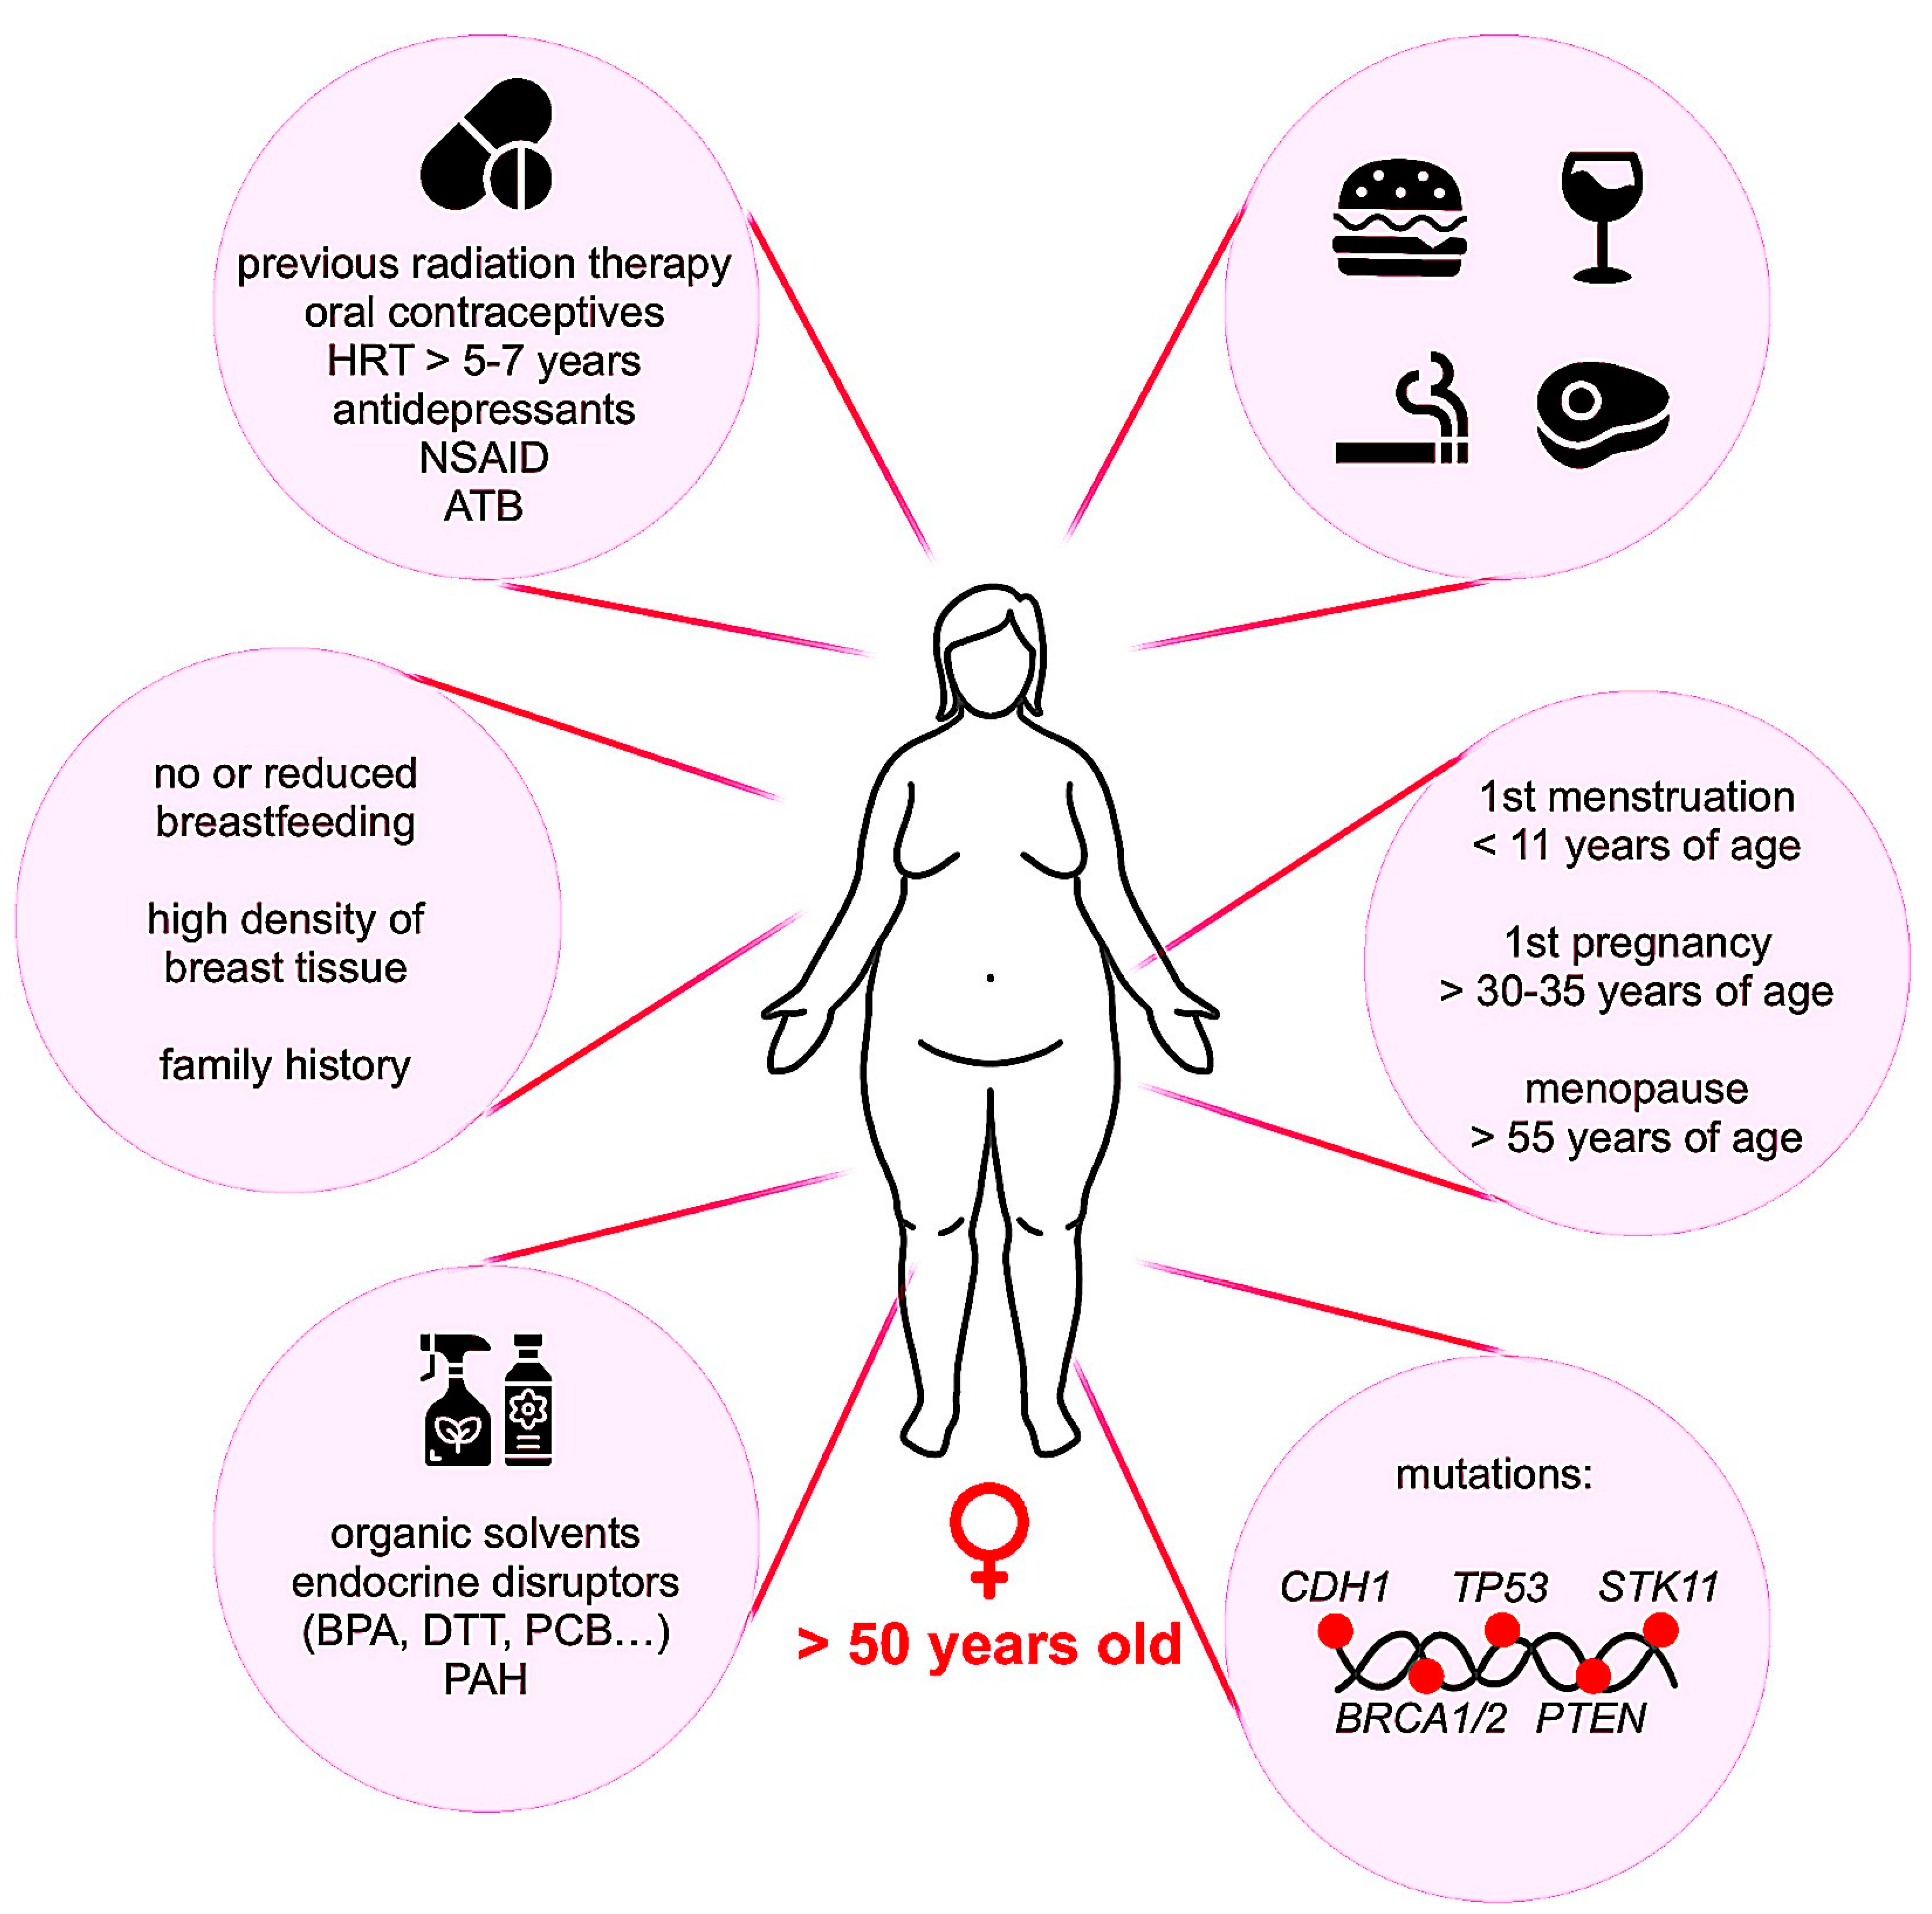
\includegraphics[width=0.7\textwidth]{chapters/2_background/figures/risk-factors.png}
    \caption{Illustration of the main risk factors for breast cancer.
        Figure was extracted from \textcite{clusan_basic_2023}.
    }
    \label{fig:brca_risk-factors}
\end{figure}

\subsection{Diagnosis}
\label{sec:brca_diagnosis}

Diagnosis of breast cancer typically involves a combination of clinical
evaluation, imaging studies, and histopathological examination.
Initial assessments often include mammography, which is a critical screening
tool that can detect tumors before they become
palpable\supercite{hameed_breast_2020}.
In cases where abnormalities are found, further imaging, such as ultrasound or
\gls{mri}, may be employed.
Definitive diagnosis is usually achieved through biopsy, where tissue samples
are collected and analyzed microscopically to confirm
malignancy\supercite{hameed_breast_2020}.
The stage at which breast cancer is diagnosed is a critical determinant of
treatment outcomes; early-stage diagnosis is associated with significantly
better prognoses\supercite{getachew_perceived_2020}.
However, barriers to early diagnosis, such as lack of awareness and access to
healthcare facilities, can lead to advanced-stage presentations, which are
linked to poorer clinical
outcomes\supercite{getachew_perceived_2020,dickens_stage_2014}.

\subsection{Treatment}
\label{sec:brca_treatment}

While type-specific treatment options have already been shown in
\cref{tab:brca_subtypes}, the choice of treatment for breast cancer is
multifaceted and depends on various factors, including the cancer subtype,
stage, and the patient's overall health.
Standard treatment modalities include surgery, radiation therapy, chemotherapy,
hormone therapy, and targeted therapies.
Surgical options may range from lumpectomy, which conserves breast tissue, to
mastectomy, which involves the removal of one or both
breasts\supercite{metcalfe_contralateral_2014,wu_breast_2014}.
Adjuvant therapies, such as chemotherapy and radiation, are often utilized to
reduce the risk of recurrence, especially in more aggressive forms like
\gls{tnbc}, which is prevalent among women with BRCA1
mutations\supercite{metcalfe_contralateral_2014}.
Hormonal therapies, such as \gls{tam} or aromatase inhibitors, are effective in
\gls{hr+} breast cancers, while targeted therapies, including \gls{her2}
inhibitors, have revolutionized treatment for \gls{her2+}
subtypes\supercite{eccles_critical_2013,pace_breast_2016}.
The choice of treatment is increasingly personalized, taking into account
genetic and epigenetic factors that may influence tumor behavior and patient
response to therapy\supercite{khakpour_methylomics_2017}.
